\documentclass[10pt]{book}
\usepackage{cite}
\usepackage{hyperref}
\usepackage{amsmath}
\usepackage{amsfonts}
\usepackage{graphicx}
\usepackage[font=small,labelfont=bf]{caption}
\hypersetup{colorlinks = true}

\author{Alberto Paoluzzi, Francesco Furiani, Giulio Martella}
\title{Linear Algebraic Representation}

\begin{document}

\frontmatter
\maketitle
\tableofcontents


\mainmatter

\documentclass[10pt]{book}
\usepackage{cite}
\usepackage{hyperref}
\usepackage{amsmath}
\usepackage{amsfonts}
\hypersetup{colorlinks = true}

\author{Alberto Paoluzzi, Francesco Furiani, Giulio Martella}
\title{Linear Algebraic Representation}

\begin{document}

\frontmatter
\maketitle
\tableofcontents

\mainmatter

\chapter{Introduction}

@O lib/jl/LARLIB.jl
@{@}


\backmatter


\bibliography{book}{}
\bibliographystyle{plain}
\end{document}

\input{ch2_spatial_arrangement.tex}
\documentclass[10pt]{book}
\usepackage{cite}
\usepackage{hyperref}
\usepackage{amsmath}
\usepackage{amsfonts}
\hypersetup{colorlinks = true}

\author{Alberto Paoluzzi, Francesco Furiani, Giulio Martella}
\title{Linear Algebraic Representation}

\begin{document}

\frontmatter
\maketitle
\tableofcontents





\mainmatter

\chapter{Planar Arrangement}

%%%%%%%%%%%%%%%%%%
\section{Overview}
Here we present the planar arrangement algorithm. It takes the 1-skeleton of the $\sigma$ face and returns complex made of 2-cells.
It puts \texttt{EVsigma} and \texttt{EVints} together into \texttt{EV} and then fragments every edge in \texttt{EV}. 
When the fragmentation is done, coincident vertices are merged into one and useless edges are deleted. At last,
2-cells are build and the result is returned.
@O lib/jl/planar_arrangement.jl
@{@< Imports and aliases @>
@< Planar arrangement support functions @>

function planar_arrangement(V::Verts, EVsigma::Cells, EVints::Cells)
    @< Local variables @>
    EV = [EVsigma; EVints]
    edgenum = size(EV, 1)
    for i in 1:edgenum
        @< Fragment edge @>
    end
    @< Put fragmentation results together @>
    @< Merge coincident vertices @>
    @< Find maximal biconnected components @>
    @< Filter biconnected components @>
    @< Create faces @>

    V, EV, FE
end 
@}
We define some aliases to standardize data formats.
@D Imports and aliases
@{typealias Verts Array{Float64, 2}
typealias Cells SparseMatrixCSC{Int8, Int}
typealias Cell SparseVector{Int8, Int}
@}
%++++++++++++++++%
\subsection{Tests}
Every function responsible for the planar arrangement is accompanied by some tests.
We start by defining a test case.
@O test/jl/planar_arrangement.jl
@{using Base.Test
include("../../lib/jl/planar_arrangement.jl")

@< Planar arrangement support functions tests @>
@< General tests @>
@}










%%%%%%%%%%%%%%%%%%%%%%%%%%%%
\section{Edge fragmentation}
%++++++++++++++++++++++++++++%
\subsection{Support functions}
%--------------------------------%
\subsubsection{Edge fragmentation}
\label{sec:frag_edge}
The edge fragmentation is performed by using a function called \texttt{frag\_edge}.
It fragments the edge of index \texttt{edgenum} into \texttt{EV} computing the intersections of
it with the other edges into \texttt{EV}. It returns the updated vertices list \texttt{V} and an 
\texttt{EV} matrix that contains the freshly computed edges.
For every edge in \texttt{EV}, it needs to check if \texttt{edge}(the edge of index \texttt{edgenum} into 
\texttt{EV}) intersects with it. This is done through \texttt{intersect\_edges} (see \ref{sec:intersect_edges}); 
this function takes two edges and returns a list of the intersections of the first edge with the second one; 
every entry of this list is a tuple made of the intersection point and a normalized intersection parameter. 
When there is an intersection, the new point is be pushed into the \texttt{V} matrix while the parameter 
is stored into the \texttt{alphas} dictionary as a key coupled to the new point index.
When every possible intersection is found, the keys in \texttt{alphas} are sorted and, on the base of that,
a new \texttt{EV} is computed.
@D Planar arrangement support functions
@{function frag_edge(V::Verts, EV::Cells, edgenum::Int)
    alphas = Dict{Float64, Int}()
    edge = EV[edgenum, :]
    for i in 1:size(EV, 1)
        if i != edgenum
            intersection = intersect_edges(V, edge, EV[i, :])
            for (point, alpha) in intersection
                V = [V; point]
                alphas[alpha] = size(V, 1)
            end
        end
    end

    alphas[0.0], alphas[1.0] = edge.nzind

    alphas_keys = sort(collect(keys(alphas)))
    cells_num = length(alphas_keys)-1
    verts_num = size(V, 1)
    EV = spzeros(Int8, cells_num, verts_num)

    for i in 1:cells_num
        EV[i, alphas[alphas_keys[i]]] = 1
        EV[i, alphas[alphas_keys[i+1]]] = 1
    end

    V, EV
end
@}
%--------------------------------%
\subsubsection{Edge intersections}
\label{sec:intersect_edges}
We used the method presented by Bourke\cite{bourke} to calculate
the intersection of two edges. Particular attention is needed on the case of colinear edges: it can happen
that \texttt{edge2} is contained into the bounds of the colinear \texttt{edge1}; in this case, both points of
\texttt{edge2} are to be considered intersection and hence must be returned. Because of this, 
the intersections are returned as a list than can contain from zero to two elements; 
each element is a couple \texttt{\{Verts, Float64\}} which represent the intersection
point and a parameter that is useful for sorting the fragmentation points of an edge.
@D Planar arrangement support functions
@{function intersect_edges(V::Verts, edge1::Cell, edge2::Cell)
    x1, y1, x2, y2 = vcat(map(c->V[c, :], edge1.nzind)...)
    x3, y3, x4, y4 = vcat(map(c->V[c, :], edge2.nzind)...)
    ret = Array{Tuple{Verts, Float64}, 1}()
    denom = (y4-y3)*(x2-x1) - (x4-x3)*(y2-y1)
    a = ((x4-x3)*(y1-y3) - (y4-y3)*(x1-x3)) / denom
    b = ((x2-x1)*(y1-y3) - (y2-y1)*(x1-x3)) / denom
    
    if 0 < a < 1 && 0 < b < 1
        p = [(x1 + a*(x2-x1))  (y1 + a*(y2-y1))]
        push!(ret, (p, a))
    elseif isnan(a) && isnan(b) 
        @< Handle colinear edges @>
    end
    return ret
end
@}

If the $\langle$ Handle colinear edges $\rangle$ macro is run, we are sure that the four vertices of 
\texttt{edge1} and \texttt{edge2} are colinear. So, to find if \texttt{edge2} has one or both of 
its vertices inside \texttt{edge1} we follow this procedure:
\begin{enumerate}
\item We parametrize \texttt{edge1}:
\[
    p = p_1 + \alpha(p_2-p_1), \quad\alpha\in[0, 1]
\]
Where $p_1$ and $p_2$ are the vertices of \texttt{edge1}
\item We solve for $\alpha$:
\begin{gather*}
    o = p_1, \quad\vec{v} = p_2 - p_1 \\
    p = o + \alpha\vec{v} \\
    p - o = \alpha\vec{v} \\
    \vec{v}^\top\cdot(p-o) = \alpha (\vec{v}^\top\cdot\vec{v}) \\
    \alpha = \frac{\vec{v}^\top\cdot(p-o)}{\vec{v}^\top\cdot\vec{v}}
\end{gather*}
\item We replace $p$ of the last equation with both the vertices of \texttt{edge2}.
If the result is $\in[0,1]$ then an intersection is found.
\end{enumerate} 
@D Handle colinear edges
@{o = [x1 y1] 
v = [x2 y2] - o
alpha = 1/dot(v,v')
ps = [x3 y3; x4 y4]
for i in 1:2
    a = alpha*dot(v',(reshape(ps[i, :], 1, 2)-o))
    if 0 < a < 1
        push!(ret, (ps[i:i, :], a))
    end
end
@}
%+++++++++++++++++++++++++%
\subsection{Implementation}
When we need to fragment an \texttt{edge} we use the \texttt{frag\_edge} function (see \ref{sec:frag_edge}) 
and we simply update \texttt{V} and push the small \texttt{ev} matrix into a list of cells called \texttt{EVs}.
We also keep the number of cells into \texttt{finalcells\_num} to build \texttt{EV} with ease.
@D Fragment edge
@{V, ev = frag_edge(V, EV, i)
finalcells_num += size(ev, 1)
push!(EVs, ev)
@}
We declare \texttt{EVs} and \texttt{finalcells\_num} as local variables of \texttt{planar\_arrangement}.
@D Local variables
@{EVs = Array{Cells, 1}()
finalcells_num = 0
@}
So now we have a \texttt{V} that contains the original points with the points computed with the fragmentation
and \texttt{EVs}, a list of edges matrices. We must now put the entries of this list together to form an unique
\texttt{EV} matrix. The process is not immediate because every entry of the list has columns relative to the 
number of vertices in \texttt{V} at the moment of the computation.
@D Put fragmentation results together
@{EV = spzeros(Int8, finalcells_num, size(V,1))
newcell_index = 1
for ev in EVs
    s = size(ev)
    EV[newcell_index:newcell_index+s[1]-1, 1:s[2]] = ev
    newcell_index += s[1]
end
@}
%++++++++++++++++%
\subsection{Tests}
@D Planar arrangement support functions tests
@{V = [0 0; 2 0; 1 1.5; -1 1; 3 1; -1 0; 3 0]
EVsigma = sparse(Array{Int8, 2}([
    [1 1 0 0 0 0 0]
    [0 1 1 0 0 0 0]
    [1 0 1 0 0 0 0]
]))
EVints = sparse(Array{Int8, 2}([
    [0 0 0 1 1 0 0]
    [0 0 0 0 0 1 1]
]))

@@testset "intersect_edges test" begin
    inters1 = intersect_edges(V, EVints[2, :], EVsigma[1, :])
    inters2 = intersect_edges(V, EVsigma[1, :], EVints[1, :])
    inters3 = intersect_edges(V, EVsigma[1, :], EVsigma[2, :])
    @@test inters1 == [([0. 0.], 1/4),([2. 0.], 3/4)]
    @@test inters2 == []
    @@test inters3 == []
end

@@testset "frag_edge test" begin
    rV, rEV = frag_edge(V, [EVsigma; EVints], 5)
    @@test rV == [V; [0 0; 2 0]]
    @@test full(rEV) == [
        [0 0 0 0 0 1 0 1 0]
        [0 0 0 0 0 0 0 1 1]
        [0 0 0 0 0 0 1 0 1]
    ]
end
@}






%%%%%%%%%%%%%%%%%%%%%%%%%%%%%%%%%%%
\section{Coincident vertices merge}
%++++++++++++++++++++++++++++%
\subsection{Support function}
\label{sec:merge_vertices}
The merge of coincident is done in the \texttt{merge\_vertices}
function. This relies on the \texttt{NearestNeighbors.jl} package\cite{NearestNeighbors}
which provides a reliable implementation of the \texttt{KDTree} data structure.
@D Imports and aliases
@{using NearestNeighbors
@}
@D Planar arrangement support functions
@{function merge_vertices(V::Verts, EV::Cells, err=1e-10)
    kdtree = KDTree(V')
    tocheck = collect(size(V,1):-1:1)
    todelete = Array{Int64, 1}()
    @< Iterate over tocheck @>
    @< Delete vertices in todelete @>
    @< Delete superfluous cells @>
    V,EV
end
@}
We create two stacks: \texttt{tocheck} which contains the indices of the vertices
to check and \texttt{todelete} that stores the indices of the vertices to delete later.
Into \texttt{tocheck} we put all the vertices of the complex in reverse order (in
this way we can pop from the stack the indices in crescent order). So, until \texttt{tocheck} is not empty,
we pop a vertex \texttt{vi} from the stack and for each coincident vertex \texttt{vj}, we put it 
into the \texttt{todelete} stack and we sum the columns of \texttt{EV} relative to \texttt{vi} and \texttt{vj}
@D Iterate over tocheck 
@{while !isempty(tocheck)
    vi = pop!(tocheck)
    if !(vi in todelete)
        nearvs = inrange(kdtree, V[vi, :], err)
        for vj in nearvs
            if vj != vi
                push!(todelete, vj)
                EV[:,vi] = EV[:, vi] + EV[:, vj]
            end
        end
    end
end
@}
We then calculate the vertices to keep and we filter out
the data relative to the vertices into \texttt{todelete}.
@D Delete vertices in todelete
@{tokeep = setdiff(collect(1:size(V,1)), todelete)
EV = EV[:, tokeep]
V = V[tokeep, :]
@}
At last we delete duplicated, empty and broken edges.
@D Delete superfluous cells
@{tokeep = Array{Int64, 1}()
cells = [Set(EV[i, :].nzind) for i in size(EV,1):-1:1]
i = 0
while !isempty(cells)
    i += 1
    c = pop!(cells)
    if !(length(c) != 2 || c in cells)
        push!(tokeep, i)
    end
end
EV = EV[tokeep, :]
@}
%+++++++++++++++++++++++++%
\subsection{Implementation}
We simply call \texttt{merge\_vertices} (see \ref{sec:merge_vertices}).
@D Merge coincident vertices
@{V, EV = merge_vertices(V, EV)
@}
%++++++++++++++++%
\subsection{Tests}
@D Planar arrangement support functions tests
@{
n0 = 1e-12
n1l = 1-1e-12
n1u = 1+1e-12
V = [
    [n0 n0; -n0 n0; n0 -n0; -n0 -n0]
    [n0 n1u; -n0 n1u; n0 n1l; -n0 n1l]
    [n1u n1u; n1l n1u; n1u n1l; n1l n1l]
    [n1u n0; n1l n0; n1u -n0; n1l -n0]
]
EV = sparse(Array{Int8, 2}([
    [1 0 0 0 1 0 0 0 0 0 0 0 0 0 0 0]
    [0 1 0 0 0 1 0 0 0 0 0 0 0 0 0 0]
    [0 0 1 0 0 0 1 0 0 0 0 0 0 0 0 0]
    [0 0 0 1 0 0 0 1 0 0 0 0 0 0 0 0]
    [0 0 0 0 1 0 0 0 1 0 0 0 0 0 0 0]
    [0 0 0 0 0 1 0 0 0 1 0 0 0 0 0 0]
    [0 0 0 0 0 0 1 0 0 0 1 0 0 0 0 0]
    [0 0 0 0 0 0 0 1 0 0 0 1 0 0 0 0]
    [0 0 0 0 0 0 0 0 1 0 0 0 1 0 0 0]
    [0 0 0 0 0 0 0 0 0 1 0 0 0 1 0 0]
    [0 0 0 0 0 0 0 0 0 0 1 0 0 0 1 0]
    [0 0 0 0 0 0 0 0 0 0 0 1 0 0 0 1]
    [1 0 0 0 0 0 0 0 0 0 0 0 1 0 0 0]
    [0 1 0 0 0 0 0 0 0 0 0 0 0 1 0 0]
    [0 0 1 0 0 0 0 0 0 0 0 0 0 0 1 0]
    [0 0 0 1 0 0 0 0 0 0 0 0 0 0 0 1]
]))
V, EV = merge_vertices(V, EV)
@@testset "merge_vertices test" begin
    @@test V == [n0 n0; n0 n1u; n1u n1u; n1u n0]
    @@test full(EV) == [
        [1 1 0 0]
        [0 1 1 0]
        [0 0 1 1]
        [1 0 0 1]
    ]
end
@}




%%%%%%%%%%%%%%%%%%%%%%%%%%%%%%%%%%%%%%%%
\section{Maximal biconnected components}
%+++++++++++++++++++++++++++%
\subsection{Support function}
\label{sec:biconnected_components}
To individuate the maximal biconnected components of the fragmented and merged 1-skeleton
we use the well know 1973 Hopcroft-Tarjan algorithm for biconnected components\cite{Hopcroft-Tarjan}.
@D Planar arrangement support functions
@{function biconnected_components(EV::Cells)
    @< Declare local variables @>
    @< DFS utilities @>
    @< Depth first visit @>
    bicon_comps
end
@}
We will need a point stack (\texttt{ps}), an edge stack (\texttt{es}), a list of traversed edges (\texttt{todel}), a list of 
visited points (\texttt{visited}), a list of biconnected components (\texttt{bicon\_comps}) and a index to avoid duplicate 
numbering of vertices (\texttt{hivtx}). \texttt{ps} is made of triples composed by the index of the vertex in \texttt{V}, 
the index assigned by the algorithm and the component identifier also assigned by the algorithm. \texttt{es} instead 
contains couples with the index of the edge inside \texttt{EV} and the assigned index of the tail node. The indexes 
in \texttt{todel} and \texttt{bicon\_comps} are relative to \texttt{EV} while the ones of \texttt{visited} are
relative to \texttt{V}
@D Declare local variables
@{ps = Array{Tuple{Int, Int, Int}, 1}()
es = Array{Tuple{Int, Int}, 1}()
todel = Array{Int, 1}()
visited = Array{Int, 1}()
bicon_comps = Array{Array{Int, 1}, 1}()
hivtx = 1
@}
Here are implemented some functions helpful throughout the algorithm.
\texttt{an\_edge} returns the index relative to \texttt{EV} of the first edge out of \texttt{point} if exists or 
\texttt{false} otherwise. \texttt{get\_head}, given an \texttt{edge} and a point (the \texttt{tail}), returns the 
index relative to \texttt{V} of the head (the point that is not \texttt{tail}) of the \texttt{edge}. 
\texttt{v\_to\_vi}, given the index relative to \texttt{V} of a vertex (\texttt{v}), returns its index using 
the algorithm numbering. This index can also not exists; in this case \texttt{false} is returned.
@D DFS utilities
@{function an_edge(point)
    edges = setdiff(EV[:, point].nzind, todel)
    if length(edges) == 0
        edges = [false]
    end
    edges[1]
end

function get_head(edge, tail)
    setdiff(EV[edge, :].nzind, [tail])[1]
end

function v_to_vi(v)
    i = findfirst(t->t[1]==v, ps)
    if i == 0
        return false
    else
        return ps[i][2]
    end
end
@}
The DFS visit is mostly akin to the one proposed in the Hopcroft-Tarjan original algorithm.
The starting point is the first one in \texttt{V}.
@D Depth first visit
@{push!(ps, (1,1,1))
push!(visited, 1)
exit = false
while !exit
    edge = an_edge(ps[end][1])
    if edge != false
        tail = ps[end][2]
        head = get_head(edge, ps[end][1])
        hi = v_to_vi(head)
        if hi == false
            hivtx += 1
            push!(ps, (head, hivtx, ps[end][2]))
            push!(visited, head)
        else
            if hi < ps[end][3]
                ps[end] = (ps[end][1], ps[end][2], hi)
            end
        end
        push!(es, (edge, tail))
        push!(todel, edge)
    else
        if length(ps) == 1
            @< Handle disconnected graph @>
        else
            if ps[end][3] == ps[end-1][2]
                @< Form biconnected component @>
            else
                if ps[end-1][3] > ps[end][3]
                    ps[end-1] = (ps[end-1][1], ps[end-1][2], ps[end][3])
                end
            end
            pop!(ps)
        end
    end
end
@}
To form a biconnected component we pop edges out from the stack of edges (\texttt{es}) until we find the one
of which the index of its tail is equal to the component identifier (called \texttt{LOWPOINT} in the original algorithm) 
of the top point of the point stack (\texttt{ps}). We effectively put inside the \texttt{bicon\_comps} only the components
made of more than one edge because we are interested in building a 1-skeleton of valid 2-cells.
@D Form biconnected component
@{edges = Array{Int, 1}()
while true
    edge, tail = pop!(es)
    push!(edges, edge)
    if tail == ps[end][3]
        if length(edges) > 1
            push!(bicon_comps, edges)
        end
        break
    end
end
@}
When there are no more points to visit in the current connected component we search for a point in \texttt{V}
which has not been visited yet (so a point not listed in the \texttt{visited} array) and we put it on the top
of a new point stack and then let the algorithm iterate again. If there are no more new connected components 
to visit we break the algorithm iteration and exit.
@D Handle disconnected graph
@{found = false
pop!(ps)
for i in 1:size(EV,2)
    if !(i in visited)
        hivtx = 1
        push!(ps, (i, hivtx, 1))
        push!(visited, i)
        found = true
        break
    end
end
if !found
    exit = true
end
@}
%+++++++++++++++++++++++++%
\subsection{Implementation}
Like for the vertices merge we simply call the freshly implemented \texttt{biconnected\_components} function
(see \ref{sec:biconnected_components}).
@D Find maximal biconnected components
@{bicon_comps = biconnected_components(EV)
@}
We also need to delete edges that are not part of a maximal biconnected component.
Once we delete the cells, we also need to check if there are isolated vertices and then
delete them from both \texttt{V} and \texttt{EV}.
@D Filter biconnected components
@{EV = EV[union(bicon_comps...), :]
vertinds = 1:size(EV, 2)
todel = Array{Int64, 1}()
for i in vertinds
    if length(EV[:, i].nzind) == 0
        push!(todel, i)
    end
end
tokeep = setdiff(vertinds, todel)
EV = EV[:, tokeep]
V = V[tokeep, :]
@}
%++++++++++++++++%
\subsection{Tests}
@D Planar arrangement support functions tests
@{EV = sparse(Array{Int8, 2}([
    [1 0 0 0 0 0 1 0 0 0 0 0]   #1
    [1 0 0 1 0 0 0 0 0 0 0 0]   #2
    [0 0 0 1 1 0 0 0 0 0 0 0]   #3
    [0 0 0 0 1 0 1 0 0 0 0 0]   #4
    [0 1 0 0 0 1 0 0 0 0 0 0]   #5
    [0 1 0 0 0 0 0 1 0 0 0 0]   #6
    [0 0 1 0 0 0 0 1 0 0 0 0]   #7
    [0 0 1 0 0 1 0 0 0 0 0 0]   #8
    [0 0 0 0 0 0 1 0 1 0 0 0]   #9
    [0 0 0 0 0 0 0 0 1 1 0 0]   #10
    [0 0 0 0 0 0 0 0 1 0 1 0]   #11
    [0 0 0 0 0 0 0 0 1 0 0 1]   #12
]))

bc = biconnected_components(EV)
bc = Set(map(Set, bc))
@@testset "biconnected_components test" begin
    @@test bc == Set([Set([1,2,3,4]), Set([5,6,7,8])])
end
@}




%%%%%%%%%%%%%%%%%%%%%%%%
\section{Faces creation}
%+++++++++++++++++++++++++++%
\subsection{Support function}
\label{sec:create_faces}

As last step, we need to compute the boundary of the 2-faces.
To do that we define the \texttt{create\_faces}.

@D Planar arrangement support functions
@{function create_faces(V::Verts, EV::Cells)
    edgenum, vertsnum = size(EV)
    edge_markers = zeros(Int8, edgenum)
    edge_angles = Array{Array{Int64, 1}, 1}(vertsnum)
    FE = zeros(Int8, 0, edgenum)
    @< Faces creation utilities @>

    @< Compute edge angles @>

    while (e = get_starting_edge()) > 0
        face = zeros(Int8, edgenum)
        if edge_markers[e] == 0
            startv, oldv = EV[e, :].nzind
        else
            oldv, startv = EV[e, :].nzind
        end
        v = -1
        edge_markers[e] += 1
        face[e] = sign(oldv - startv)
        while v != startv
            e = next_edge(oldv, e)
            v = setdiff(EV[e, :].nzind, [oldv])[1]
            face[e] = sign(v - oldv)
            oldv = v
            edge_markers[e] += 1
        end
        FE = [FE; reshape(face, 1, edgenum)]
    end

    sparse(FE)
end
@}
The \texttt{get\_starting\_edge} function returns the first edge
marked with zero. If there are no edges marked with zero, the first edge
marked with one will be returned. If every edge is marked with 2 then $-1$
will be returned.
@D Faces creation utilities
@{function get_starting_edge()
    e = -1
    for i in 1:edgenum
        if edge_markers[i] == 0
            return i
        elseif edge_markers[i] == 1 && e < 0
            e = i
        end
    end
    e
end
@}

We define a function to compute the angle between an edge and the 
$x_1$-axis and we apply it to every edge out of every vertex.
The angles relative to a single vertex are then sorted in counterclockwise order.

@D Compute edge angles
@{function edge_angle(v::Int, edge::Cell)
    v2 = setdiff(edge.nzind, [v])[1]
    x, y = V[v2, :] - V[v, :]
    return atan2(y, x)
end

for v in 1:vertsnum
    as = [(e, edge_angle(v, EV[e, :])) for e in EV[:, v].nzind]
    sort!(as, lt=(a,b)->a[2]<b[2])
    as = map(a->a[1], as)
    edge_angles[v] = as
end
@}

The \texttt{next\_edge} function determines the next edge to visit
while building a face. It needs a vertex index (\texttt{v}) and 
an edge index (\texttt{e}) as input.

@D Faces creation utilities
@{function next_edge(v::Int64, e::Int64)
    angles = edge_angles[v]
    ne = findfirst(angles, e)
    while true
        ne += 1
        if ne > length(angles)
            ne = 1
        end
        if edge_markers[angles[ne]] < 2
            break
        end
    end
    angles[ne]
end
@}

%++++++++++++++++%
\subsection{Implementation}
Back in the \texttt{planar\_arrangement} function, we simply store the signed boundary matrix.
@D Create faces
@{FE = create_faces(V, EV)
@}

%++++++++++++++++%
\subsection{Tests}
@D Planar arrangement support functions tests
@{@@testset "create_faces test" begin
    V = [0 0; 1 1; -1 1; -1 -1; 1 -1.]
    EV = sparse(Array{Int8, 2}([
        [1 1 0 0 0]
        [1 0 1 0 0]
        [1 0 0 1 0]
        [1 0 0 0 1]
        [0 1 1 0 0]
        [0 0 1 1 0]
        [0 0 0 1 1]
        [0 1 0 0 1]
    ]))

    FE = create_faces(V, EV)
    
    @@test FE == sparse(Array{Int8, 2}([
        [1 0 0 -1 0 0 0 1] 
        [-1 1 0 0 -1 0 0 0]
        [0 -1 1 0 0 -1 0 0]
        [0 0 0 0 1 1 1 -1]
        [0 0 -1 1 0 0 -1 0]
    ]))
end
@}








%%%%%%%%%%%%%%%%%%%%%%%
\section{General tests}

Here we present some general tests for the \texttt{planar\_arrangement} function

%+++++++++++++++++%
\subsection{Test 1}
@D General tests
@{@@testset "General test #1" begin
    V = [0 0; 2 0; 1 1.5; -1 1; 3 1; -1 0; 3 0]
    EVsigma = sparse(Array{Int8, 2}([
        [1 1 0 0 0 0 0]
        [0 1 1 0 0 0 0]
        [1 0 1 0 0 0 0]
    ]))
    EVints = sparse(Array{Int8, 2}([
        [0 0 0 1 1 0 0]
        [0 0 0 0 0 1 1]
    ]))

    V, EV, FE = planar_arrangement(V, EVsigma, EVints)
    err = 1e-5
    @@test all(map((a,b)->-err<a-b<+err, V, [
        [0.0 0.0]
        [2.0 0.0]
        [1.0 1.5]
        [1.33333 1.0]
        [0.666667 1.0]
    ]))
    @@test EV == [0 0 0 1 1; 1 1 0 0 0; 0 1 0 1 0; 0 0 1 1 0; 0 0 1 0 1; 1 0 0 0 1]
    @@test FE == [1 0 0 1 -1 0; 0 1 1 -1 1 -1; -1 -1 -1 0 0 1]
end
@}

%+++++++++++++++++%
\subsection{Test 2}
@D General tests
@{@@testset "General test #2" begin
    V = [
        [0 0]
        [1 0]
        [1 1]
        [0 1]
        [-.05 .5]
        [1.05 .5]
        [.5 .55]
        [.5 -.05]
        [.45 .25]
        [1.05 .25]
        [.75 .3]
        [.75 -.05]
    ]
    EVsigma = sparse(Array{Int8, 2}([
        [1 1 0 0 0 0 0 0 0 0 0 0]
        [0 1 1 0 0 0 0 0 0 0 0 0]
        [0 0 1 1 0 0 0 0 0 0 0 0]
        [1 0 0 1 0 0 0 0 0 0 0 0]
    ]))
    EVints = sparse(Array{Int8, 2}([
        [0 0 0 0 1 1 0 0 0 0 0 0]
        [0 0 0 0 0 0 1 1 0 0 0 0]
        [0 0 0 0 0 0 0 0 1 1 0 0]
        [0 0 0 0 0 0 0 0 0 0 1 1]
    ]))

    V, EV, FE = planar_arrangement(V, EVsigma, EVints)
    err = 1e-5
    @@test all(map((a,b)->-err<a-b<+err, V, 
        [0 0; 1 0; 1 1; 0 1; .5 0; .75 0; 1 .5; 1 .25; 0 .5; .5 .5; .5 .25; .75 .25]))
    @@test EV == [
        [0 0 0 0 0 1 0 0 0 0 0 1]
        [0 0 0 0 0 0 0 1 0 0 0 1]
        [0 0 0 0 0 0 0 0 0 0 1 1]
        [0 0 0 0 1 0 0 0 0 0 1 0]
        [0 0 0 0 0 0 0 0 0 1 1 0]
        [0 0 0 0 0 0 1 0 0 1 0 0]
        [0 0 0 0 0 0 0 0 1 1 0 0]
        [1 0 0 0 0 0 0 0 1 0 0 0]
        [0 0 0 1 0 0 0 0 1 0 0 0]
        [0 0 1 1 0 0 0 0 0 0 0 0]
        [0 0 1 0 0 0 1 0 0 0 0 0]
        [0 0 0 0 0 0 1 1 0 0 0 0]
        [0 1 0 0 0 0 0 1 0 0 0 0]
        [0 1 0 0 0 1 0 0 0 0 0 0]
        [0 0 0 0 1 1 0 0 0 0 0 0]
        [1 0 0 0 1 0 0 0 0 0 0 0]
    ]
    @@test FE == [
        [1 -1 0 0 0 0 0 0 0 0 0 0 -1 1 0 0]
        [-1 0 1 1 0 0 0 0 0 0 0 0 0 0 -1 0]
        [0 0 0 -1 1 0 1 1 0 0 0 0 0 0 0 -1]
        [0 0 0 0 0 1 -1 0 -1 -1 1 0 0 0 0 0]
        [0 1 -1 0 -1 -1 0 0 0 0 0 1 0 0 0 0]
        [0 0 0 0 0 0 0 -1 1 1 -1 -1 1 -1 1 1]
    ]
end
@}

%+++++++++++++++++%
\subsection{Test 3}
@D General tests
@{@@testset "General test #3" begin
    V = [
        [0 0]
        [2 0]
        [2 1]
        [1 1]
        [1 2]
        [0 2]
        [1.5 0]
        [1.5 1.5]
        [0 1.5]
    ]

    EVsigma = sparse(Array{Int8, 2}([
        [1 1 0 0 0 0 0 0 0]
        [0 1 1 0 0 0 0 0 0]
        [0 0 1 1 0 0 0 0 0]
        [0 0 0 1 1 0 0 0 0]
        [0 0 0 0 1 1 0 0 0]
        [1 0 0 0 0 1 0 0 0]
    ]))
    EVints = sparse(Array{Int8, 2}([
        [1 0 0 0 0 0 1 0 0]
        [0 0 0 0 0 0 1 1 0]
        [0 0 0 0 0 0 0 1 1]
        [1 0 0 0 0 0 0 0 1]
    ]))

    V, EV, FE = planar_arrangement(V, EVsigma, EVints)
    err = 1e-5
    @@test all(map((a,b)->-err<a-b<+err, V, [
        0 0; 2 0; 2 1; 1 1; 1 2; 0 2; 1.5 0; 1.5 1.5; 0 1.5; 1.5 1; 1 1.5]))
    @@test EV == [
        [0 0 0 0 0 0 1 0 0 1 0]
        [0 0 0 0 0 0 0 1 0 1 0]
        [0 0 0 0 0 0 0 1 0 0 1]
        [1 0 0 0 0 0 0 0 1 0 0]
        [0 0 0 0 0 0 0 0 1 0 1]
        [0 0 0 0 0 1 0 0 1 0 0]
        [0 0 0 0 1 1 0 0 0 0 0]
        [0 0 0 0 1 0 0 0 0 0 1]
        [0 0 0 1 0 0 0 0 0 0 1]
        [0 0 0 1 0 0 0 0 0 1 0]
        [0 0 1 0 0 0 0 0 0 1 0]
        [0 1 1 0 0 0 0 0 0 0 0]
        [0 1 0 0 0 0 1 0 0 0 0]
        [1 0 0 0 0 0 1 0 0 0 0]
    ]
    @@test FE == [
        [1 0 0 0 0 0 0 0 0 0 -1 -1 1 0]
        [0 1 -1 0 0 0 0 0 1 -1 0 0 0 0]
        [-1 0 0 1 1 0 0 0 -1 1 0 0 0 -1]
        [0 -1 1 -1 0 1 1 -1 0 0 1 1 -1 1]
        [0 0 0 0 -1 -1 -1 1 0 0 0 0 0 0]
    ]
end
@}



\backmatter


\bibliography{book}{}
\bibliographystyle{plain}
\end{document}

\chapter{Dimension travel}

%%%%%%%%%%%%%%%%%%
\section{Overview}
@O lib/jl/dimension_travel.jl
@{@< Imports and aliases @>
@< Dimension travel functions @>
@}

@D Imports and aliases
@{include("./utilities.jl")
@}
%+++++++++++++%
\subsection{Tests}
@O test/jl/dimension_travel.jl
@{using Base.Test
include("../../lib/jl/dimension_travel.jl")

@< Tests @>
@}


%%%%%%%%%%%%%%%%%%%%%%%
\section{Normalization}
This function returns the direct and inverse transformation that
normalizes every point in \texttt{V} to mek them fit into the unitary
$d$-dimensional hyper-cube.
First of all, the function computes the bounding box of the input points.
Then it combines a translation and a scaling matrix. Lastly, it
inverts the matrix and returns both the direct and the inverse matrix.
@D Dimension travel functions
@{function normalizer(V::Verts)
    d = size(V, 2)
    upper = mapslices(x->max(x...), V, 1)
    lower = mapslices(x->min(x...), V, 1)
    diff = upper-lower

    T = eye(d+1)
    T[d+1, 1:d] = -lower

    S = eye(d+1)
    S[1:d, 1:d] = diagm(vec(map(inv, diff)))

    mat = T*S
    mat, inv(mat)
end
@}


%%%%%%%%%%%%%%%%%%%%%%%%%%%%%
\section{Submanifold mapping}

This function, given three points (in $\mathbb{E}^3$), 
returns a $4\times4$ transformation matrix that "flattens"
plane on which the points lay on the $x_3=0$ plane. 
The matrix is made of the composition of
a translation matrix and a coordinate reference change. The translation
makes the first point passes coincident to the origin and
the coordinate reference change is computed by building a reference
system of the plane define by the three points.

@D Dimension travel functions
@{function submanifold_mapping(p1, p2, p3)
    u1 = p2-p1
    u2 = p3-p1
    u3 = cross(u1, u2)
    T = eye(4)
    T[4, 1:3] = -p1
    M = eye(4)
    M[1:3, 1:3] = [u1 u2 u3]
    return T*M
end
@}
%----------------%
\subsection{Tests}

@D Tests
@{V = rand(3, 3)
face = sparsevec(Int8[1 1 1])
m = submanifold_mapping(V, face)
err = 1e-10 
@@testset "submanifold_mapping test" begin
    @@test any(map((x,y)->-err<x-y<err, m*inv(m), eye(4)))
    @@test any(x->-err<x<err, ([V [1; 1; 1]]*m)[:, 3])
end
@}





%%%%%%%%%%%%%%%%%%%%%%%%%%%%%%%%%%%
\section{Spatial index computation}

The aim of this function is to compute a \textit{spatial index} that maps
each cell to a set of cells which it may collide with.
This is achieved by profuse use of bounding boxes and interval trees. 
These last ones are implemented with the \texttt{IntervalTrees.jl} package
(\url{https://github.com/BioJulia/IntervalTrees.jl})

@D Imports and aliases
@{using IntervalTrees
@}

@D Dimension travel functions
@{function spatial_index(V::Verts, EV::Cells, FE::Cells)
    d = 3
    faces_num = size(FE, 1)
    @< Build the d-IntervalTrees @>
    @< Create the mapping @>
    mapping
end
@}

The basic idea is to "unfold" every $d$-dimensional bounding box into $d$ one-dimensional boxes.
To do so, one interval tree per dimension must be created. 
We build the $d$-trees by firstly building the intervals for each box and then the trees.
In this way we keep in memory the \texttt{boxes1D} array (which contains the intervals) for later use.

@D Build the d-IntervalTrees
@{IntervalsType = IntervalValue{Float64, Int64}
boxes1D = Array{IntervalsType, 2}(0, d)
for fi in 1:faces_num
    vidxs = (abs(FE[fi:fi,:])*abs(EV))[1,:].nzind
    intervals = map((l,u)->IntervalsType(l,u,fi), bbox(V[vidxs, :])...)
    boxes1D = vcat(boxes1D, intervals)
end
trees = mapslices(IntervalTree{Float64, IntervalsType}, sort(boxes1D, 1), 1)
@}

The \textit{spatial index} is returned as an array of \texttt{Int64} arrays.
The \texttt{intersect\_intervals} function returns every cell of which its bounding box collides with 
the $d$-intervals passed as argument. This function then is called for the $d$-intervals (stored in the \texttt{boxes1D} array) of every cell.
Obviously every cell collides with itself, so a set difference is performed for every cell to exclude itself from the mapping.

@D Create the mapping
@{function intersect_intervals(intervals)
    cells = Array{Int64,1}[]
    for axis in 1:d
        vs = map(i->i.value, intersect(trees[axis], intervals[axis]))
        push!(cells, vs)
    end
    mapreduce(x->x, intersect, cells)
end

mapping = Array{Int64,1}[]
for fi in 1:faces_num
    cell_indexes = setdiff(intersect_intervals(boxes1D[fi, :]), [fi])
    push!(mapping, cell_indexes)
end
@}


%%%%%%%%%%%%%%%%%%%%%%%%%%%%%%%%%%%%%%%%%%%%
\section{Face intersection with $z=0$ plane}

The intersection of a polygonal face with the $z=0$ computes
zero, ono or more edges. To perform the intersection we find the
intersection point of every edge with the $z=0$ plane and then
we connect the points.

@D Dimension travel functions
@{function face_int(V::Verts, EV::Cells, face::Cell)

    vs = buildFV(EV, face)
    retV = Verts(0, 3)

    for i in 1:length(vs)
        o = V[vs[i],:]
        j = i < length(vs) ? i+1 : 1
        d = V[vs[j],:] - o

        alpha = -o[3] / d[3]

        if 0 < alpha < 1
            p = o + alpha*d
            retV = [retV; reshape(p, 1, 3)]
        end

    end

    vnum = size(retV, 1)
    enum = Int(vnum / 2)
    retEV = spzeros(Int8, enum, vnum)

    for i in 1:enum
        retEV[i, 2*i-1:2*i] = [-1, 1]
    end

    retV, retEV
end
@} 

\chapter{Minimal cycles computation}
\label{ch:minimal_cycles}

\section{Main function}


Computing the minimal cycles means to compute the $d$-boundary matrix
from the $(d-1)$-boundary. This function works for both $d=2$ and $d=3$;
the only difference between the two cases lays in the \texttt{angles\_fn}
function (ref. \ref{sec:angles_fn}). To support this multidimensional
behavior, the algorithm has been implemented as an high-order function\footnote{
    \textbf{Notes on variables names:} \texttt{ld} stands for \textit{lower dimension} ($d-1$)
    and \texttt{lld} for \textit{lower lower dimension} ($d-2$). So, \texttt{ld\_cellsnum} is the
    short form of \textit{lower dimension cell number}. For example, if $d=2$, \texttt{ld\_cellsnum} stands for the
    number of $1-$cells, aka the edges.
}:

@O lib/jl/minimal_cycles.jl
@{include("./utilities.jl")
using TRIANGLE

@< Minimal cycles implementations @>

function minimal_cycles(angles_fn::Function)

    function _minimal_cycles(V::Verts, ld_bounds::Cells)
        @< Function body @>
    end

    return _minimal_cycles
end
@}

In the internal function we store an array of integers called \texttt{count\_marks} 
that increments every time a cells is visited. We do that because to build 
a complete $d$-boundary, we must visit every $(d-1)$-cell exactly twice;
Said so, it appears clear that the algorithm must iterate until a $(d-1)$-cell 
marked with 0 or 1 can be found. Near to \texttt{count\_marks} is stored another
array called \texttt{dir\_marks} that memorizes the direction in which each $(d-1)$-cell
has been visited the last time (this is useful to determine the direction in which the cell
must be visited next)

@D Function body
@{lld_cellsnum, ld_cellsnum = size(ld_bounds)
count_marks = zeros(Int8, ld_cellsnum)
dir_marks = zeros(Int8, ld_cellsnum)
d_bounds = spzeros(Int8, ld_cellsnum, 0)

@< minimal\_cycles local variables @>
@< minimal\_cycles utilities @>

while (sigma = get_seed_cell()) > 0
    println("sigma: ", sigma)
    @< Compute a cycle @>
end

return d_bounds
@}

The \texttt{get\_seed\_cell} function returns the first $d-1$ cell
marked with zero. If there are no cells marked with zero, the first cell
marked with one will be returned. If every cell is marked with 2 then $-1$
will be returned.

@D minimal\_cycles utilities
@{function get_seed_cell()
    s = -1
    for i in 1:ld_cellsnum
        if count_marks[i] == 0
            return i
        elseif count_marks[i] == 1 && s < 0
            s = i
        end
    end
    return s
end
@}

The bigger part of the algorithm is the computation
of a single cycle. It is mostly equivalent to the
\textbf{ALGORITHM 1} presented by A. Paoluzzi et al.
in \textit{Arrangements of cellular complexes}
\cite{Paoluzzi}

@D Compute a cycle
@{c_ld = spzeros(Int8, ld_cellsnum)
if count_marks[sigma] == 0
    c_ld[sigma] = 1
else
    c_ld[sigma] = -dir_marks[sigma]
end
c_lld = ld_bounds*c_ld
while c_lld.nzind != []
    corolla = spzeros(Int8, ld_cellsnum)
    for tau in c_lld.nzind
        b_ld = ld_bounds[tau, :]
        pivot = intersect(c_ld.nzind, b_ld.nzind)[1]
        adj = nextprev(tau, pivot, sign(-c_lld[tau]))
        corolla[adj] = c_ld[pivot]
        if b_ld[adj] == b_ld[pivot]
            corolla[adj] *= -1
        end
    end
    #=
    if sigma == 1
        println(c_ld)
        readline(STDIN)
    end
    =#
    c_ld += corolla
    c_lld = ld_bounds*c_ld
end
map(s->count_marks[s] += 1, c_ld.nzind)
map(s->dir_marks[s] = c_ld[s], c_ld.nzind)
d_bounds = [d_bounds c_ld]
@}

As profusely explained by A. Paoluzzi et al. \cite{Paoluzzi}, this algorithm
revolves around the \textit{next} and \textit{prev} functions. To speed up their
computation, before the cycles iteration starts, we calculate and
store for each ($d-2$)-cell the angles that its incident ($d-1$)-cells
form with it.

@D minimal\_cycles local variables
@{angles = Array{Array{Int64, 1}, 1}(lld_cellsnum)
@}

Here we use the parameter \texttt{angles\_fn::Function}. As explained earlier,
this function is the only difference between the $d=3$ and $d=2$ version of
\texttt{minimal\_cycles}.

@D minimal\_cycles utilities
@{
for lld in 1:lld_cellsnum
    as = []
    for ld in ld_bounds[lld, :].nzind
        push!(as, (ld, angles_fn(lld, ld)))
    end
    sort!(as, lt=(a,b)->a[2]<b[2])
    as = map(a->a[1], as)
    angles[lld] = as
end
@}

Once computed the \texttt{angles}, the \texttt{nextprev} function is
easy to implement. The \texttt{norp} parameter is a short form for \textit{next or prev}. 
It determines if the function should choose the first available
($d-1$)-cell rotating clockwise or counterclockwise around the ($d-2$)-cell.

@D minimal\_cycles utilities
@{function nextprev(lld::Int64, ld::Int64, norp)
    as = angles[lld]
    ne = findfirst(as, ld)
    while true
        ne += norp
        if ne > length(as)
            ne = 1
        elseif ne < 1
            ne = length(as)
        end

        if count_marks[as[ne]] < 2
            break
        end
    end
    as[ne]
end
@}



\section{Dimensional wise implementations}
\label{sec:angles_fn}

%%%%%%%%%%%%%%%%%%
\subsection{$d=2$}

When in $d=2$, ($d-2$)-cells are vertices and ($d-1$)-cells are edges.
The \texttt{edge\_angle} function uses the Julia's \texttt{atan2} 
built-in function to calculate the angle of the edge from the vertex point of view.

@D Minimal cycles implementations
@{function minimal_2cycles(V::Verts, EV::Cells)

    function edge_angle(v::Int, e::Int)
        edge = EV[e, :]
        v2 = setdiff(edge.nzind, [v])[1]
        x, y = V[v2, :] - V[v, :]
        return atan2(y, x)
    end

    for i in 1:EV.m
        j = min(EV[i,:].nzind...)
        EV[i, j] = -1
    end
    VE = EV'

    EF = minimal_cycles(edge_angle)(V, VE)

    return EF'
end
@}


%%%%%%%%%%%%%%%%%%
\subsection{$d=3$}

Here we have edges for ($d-2$)-cells and faces for ($d-1$)-cells.

@D Minimal cycles implementations
@{function minimal_3cycles(V::Verts, EV::Cells, FE::Cells)

    triangulated_faces = Array{Any, 1}(FE.m)

    function face_angle(e::Int, f::Int)
        if !isdefined(triangulated_faces, f)
            vs_idxs = Array{Int64, 1}()
            edges_idxs = FE[f, :].nzind
            edge_num = length(edges_idxs)
            edges = zeros(Int64, edge_num, 2)

            for (i, ee) in enumerate(edges_idxs)
                edge = EV[ee, :].nzind
                edges[i, :] = edge
                vs_idxs = union(vs_idxs, edge)
            end
            
            vs = V[vs_idxs, :]

            v1 = normalize(vs[2, :] - vs[1, :])
            v3 = [0 0 0]
            err = 1e-8
            i = 3
            while -err < norm(v3) < err
                v2 = normalize(vs[i, :] - vs[1, :])
                v3 = cross(v1, v2)
                i = i + 1
            end

            M = reshape([v1; v2; v3], 3, 3)

            vs = vs*M

            triangulated_faces[f] = TRIANGLE.constrained_triangulation(vs, vs_idxs, edges, fill(true, edge_num))
        end

        edge_vs = EV[e, :].nzind

        t = findfirst(x->edge_vs[1] in x && edge_vs[2] in x, triangulated_faces[f])
        
        # Indexes of the vertices of the triangle
        triangle = triangulated_faces[f][t]

        # Get normalized vector of hinge
        v1 = normalize(V[edge_vs[2], :] - V[edge_vs[1], :])

        # Build frame
        if abs(v1[1]) > abs(v1[2])
            invlen = 1. / sqrt(v1[1]*v1[1] + v1[3]*v1[3])
            v2 = [-v1[3]*invlen, 0, v1[1]*invlen]
        else
            invlen = 1. / sqrt(v1[2]*v1[2] + v1[3]*v1[3])
            v2 = [0, -v1[3]*invlen, v1[2]*invlen]
        end
        v3 = cross(v1, v2)

        # Build transformation matrix
        M = reshape([v1; v2; v3], 3, 3)

        # Transform
        third_v = setdiff(triangle, edge_vs)[1]
        vs = V[[edge_vs..., third_v], :]*M

        # return atan2 of 3rd with 1st
        v = vs[3, :] - vs[1, :]

        angle = atan2(v[2], v[3]) 

        return angle
    end

    EF = FE'

    FC = minimal_cycles(face_angle)(V, EF)

    return -FC'
end
@}

\chapter{Utilities}
\label{ch:utilities}

%%%%%%%%%%%%%%%%%%
\section{Overview}

The functionalities shared between all the components of LAR
are defined in here.

@O lib/jl/utilities.jl
@{@< Aliases @>
@< Utilities @>
@}

\subsection{Tests}
As usual every function has some unit tests.

@O test/jl/utilities.jl
@{using Base.Test
include("../../lib/jl/utilities.jl")

@< Utilities tests @>
@}


%%%%%%%%%%%%%%%
\section{Types}

To store vertices and cells boundary matrices, 
we use types already built in the standard Julia.
We use these aliases to standardize the types used 
throughout LAR. 

@D Aliases
@{const Verts = Array{Float64, 2}
const Cells = SparseMatrixCSC{Int8, Int}
const Cell = SparseVector{Int8, Int}
@}




%%%%%%%%%%%%%%%%%%%%%%%%
\section{Bounding boxes}
\label{sec:bboxes}

Bounding boxes are essential in many steps of many
algorithms in LAR. Here we present a method for building
and performing containment tests on n-dimensional bounding boxes.

@D Utilities
@{function bbox(vertices::Verts)
    minimum = mapslices(x->min(x...), vertices, 1)
    maximum = mapslices(x->max(x...), vertices, 1)
    minimum, maximum
end

function bbox_contains(container, contained)
    b1_min, b1_max = container
    b2_min, b2_max = contained
    all(map((i,j,k,l)->i<=j<=k<=l, b1_min, b2_min, b2_max, b1_max))
end
@}

\subsection{Tests}
\begin{figure}[h]
    \centering
    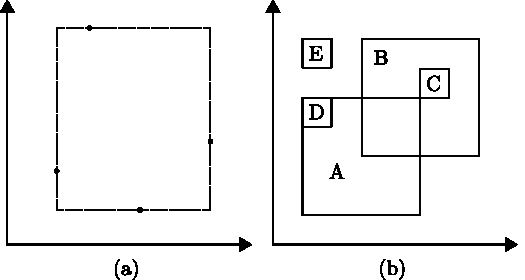
\includegraphics{./img/ch5-bboxes.pdf}
    \caption{(a) is a visualization of the test for bboxes building, (b) for bbox containment.}
\end{figure}
@D Utilities tests
@{@@testset "Bounding boxes building test" begin
    V = [.56 .28; .84 .57; .35  1.0; .22  .43]
    @@test bbox(V) == ([.22 .28], [.84 1.0])
end

@@testset "Bounding boxes containment test" begin
    bboxA = ([0. 0.], [1. 1.])
    bboxB = ([.5 .5], [1.5 1.5])
    bboxC = ([1. 1.], [1.25 1.25])
    bboxD = ([0 .75], [.25 1])
    bboxE = ([0 1.25], [.25 1.5])

    @@test bbox_contains(bboxA, bboxD)
    @@test bbox_contains(bboxB, bboxC)
    @@test !bbox_contains(bboxA, bboxB)
    @@test !bbox_contains(bboxA, bboxE)
end
@}

%%%%%%%%%%%%%%%%%%%%%%%%%%%%%%%
\section{Face area calculation}
\label{sec:face_area}

\begin{figure}[h]
    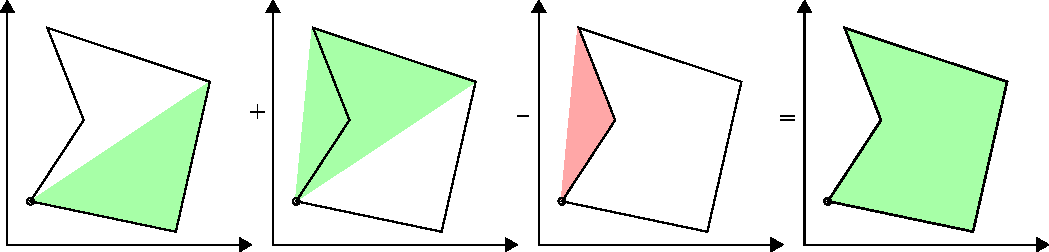
\includegraphics[width=\textwidth]{./img/ch5-area.pdf}
    \caption{A visual representation of the face area calculation algorithm. The area
    of the face is the sum of the areas of each triangle which can be build using the 
    pivot vertex and the other vertices of the face}
\end{figure}
\noindent
To compute the area of a generic (convex or concave) face,
we pick a pivot vertex of the face and then we iterate over
every edge of the face calculating the area of the triangle
made by the pivot vertex and the ordered extremes of the current edge.
The area of the full face is the sum of the areas of the single triangles.
This works because of the single triangles we compute the signed area with
this formula:
\begin{gather*}
    A = \frac{1}{2}
    \begin{vmatrix}
        p_{1x} & p_{1y} & 1 \\
        p_{2x} & p_{2y} & 1 \\
        p_{3x} & p_{3y} & 1
    \end{vmatrix}
\end{gather*}
Where $p_1$, $p_2$ and $p_3$ are the vertices of the triangle ($p_1$ is the pivot vertex). 
Please notice that the result of this formula will be negative only if these vertices 
are arranged in clockwise order.

@D Utilities
@{function face_area(V::Verts, EV::Cells, face::Cell)
    function triangle_area(triangle_points::Verts)
        ret = ones(3,3)
        ret[:, 1:2] = triangle_points
        return .5*det(ret)
    end

    area = 0
    ps = [0, 0, 0]

    for i in face.nzind
        edge = face[i]*EV[i, :]
        skip = false

        for e in edge.nzind
            if e != ps[1]
                if edge[e] < 0
                    if ps[1] == 0
                        ps[1] = e
                        skip = true
                    else
                        ps[2] = e
                    end
                else
                    ps[3] = e
                end
            else
                skip = true
                break
            end
        end

        if !skip
            area += triangle_area(V[ps, :])
        end
    end

    return area
end
@}

\subsection{Tests}
\begin{figure}[h]
    \centering
    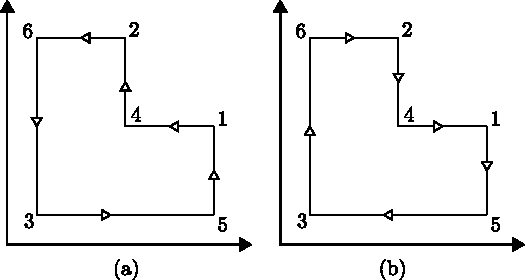
\includegraphics{./img/ch5-area_test.pdf}
\end{figure}
\noindent The two faces drawn above they must have complimentary area.
@D Utilities tests
@{@@testset "Face area calculation test" begin
    V = Float64[2 1; 1 2; 0 0; 1 1; 2 0; 0 2]
    EV = spzeros(Int8, 6, 6)
    EV[1, [1, 4]] = [-1, 1]; EV[2, [2, 4]] = [-1, 1]
    EV[3, [2, 6]] = [-1, 1]; EV[4, [3, 6]] = [-1, 1]
    EV[5, [3, 5]] = [-1, 1]; EV[6, [1, 5]] = [-1, 1]
    FE = spzeros(Int8, 2, 6)
    FE[1, :] = [ 1 -1  1 -1  1 -1]
    FE[2, :] = [-1  1 -1  1 -1  1]

    @@test face_area(V, EV, FE[1,:]) == -face_area(V, EV, FE[2,:])
end
@}

%%%%%%%%%%%%%%%%%%%%%%%%
\section{Skeletal merge}

It is generally useful to have a utility to merge the skeletons of
two cellular complexes. We have both the $d=2$ and $d=3$ versions.

@D Utilities
@{function skel_merge(V1::Verts, EV1::Cells, V2::Verts, EV2::Cells)
    V = [V1; V2]
    EV = spzeros(Int8, EV1.m + EV2.m, EV1.n + EV2.n)
    EV[1:EV1.m, 1:EV1.n] = EV1
    EV[EV1.m+1:end, EV1.n+1:end] = EV2
    V, EV
end

function skel_merge(V1::Verts, EV1::Cells, FE1::Cells, V2::Verts, EV2::Cells, FE2::Cells)
    FE = spzeros(Int8, FE1.m + FE2.m, FE1.n + FE2.n)
    FE[1:FE1.m, 1:FE1.n] = FE1
    FE[FE1.m+1:end, FE1.n+1:end] = FE2
    V, EV = skel_merge(V1, EV1, V2, EV2)
    V, EV, FE
end
@}

%%%%%%%%%%%%%%%%%%%%%%
\section{Point in face area}
\label{sec:point_in_face}

Point in face inclusion is performed using the algorithm
presented by A. Paoluzzi et al. (NEED TO FIND REFERENCE)

@D Utilities
@{function point_in_face(origin, V::Verts, ev::Cells)
    return pointInPolygonClassification(V, ev)(origin) == "p_in"
end

function crossingTest(new, old, status, count)
    if status == 0
        status = new
        return status, (count + 0.5)
    else
        if status == old
            return 0, (count + 0.5)
        else
            return 0, (count - 0.5)
        end
    end
end

function setTile(box)
    tiles = [[9,1,5],[8,0,4],[10,2,6]]
    b1,b2,b3,b4 = box
    function tileCode(point)
        x,y = point
        code = 0
        if y>b1 code=code|1 end
        if y<b2 code=code|2 end
        if x>b3 code=code|4 end
        if x<b4 code=code|8 end
        return code
    end
    return tileCode
end

function pointInPolygonClassification(V,EV)

    function pointInPolygonClassification0(pnt)
        x,y = pnt
        xmin,xmax,ymin,ymax = x,x,y,y
        tilecode = setTile([ymax,ymin,xmax,xmin])
        count,status = 0,0

        for k in 1:EV.m
            edge = EV[k,:]
            p1, p2 = V[edge.nzind[1], :], V[edge.nzind[2], :]
            (x1,y1),(x2,y2) = p1,p2
            c1,c2 = tilecode(p1),tilecode(p2)
            c_edge, c_un, c_int = c1$c2, c1|c2, c1&c2
            
            if (c_edge == 0) & (c_un == 0) return "p_on" 
            elseif (c_edge == 12) & (c_un == c_edge) return "p_on"
            elseif c_edge == 3
                if c_int == 0 return "p_on"
                elseif c_int == 4 count += 1 end
            elseif c_edge == 15
                x_int = ((y-y2)*(x1-x2)/(y1-y2))+x2 
                if x_int > x count += 1
                elseif x_int == x return "p_on" end
            elseif (c_edge == 13) & ((c1==4) | (c2==4))
                    status, count = crossingTest(1,2,status,count)
            elseif (c_edge == 14) & ((c1==4) | (c2==4))
                    status, count = crossingTest(2,1,status,count)
            elseif c_edge == 7 count += 1
            elseif c_edge == 11 count = count
            elseif c_edge == 1
                if c_int == 0 return "p_on"
                elseif c_int == 4 
                    status, count = crossingTest(1,2,status,count) 
                end
            elseif c_edge == 2
                if c_int == 0 return "p_on"
                elseif c_int == 4 
                    status, count = crossingTest(2,1,status,count) 
                end
            elseif (c_edge == 4) & (c_un == c_edge) return "p_on"
            elseif (c_edge == 8) & (c_un == c_edge) return "p_on"
            elseif c_edge == 5
                if (c1==0) | (c2==0) return "p_on"
                else 
                    status, count = crossingTest(1,2,status,count) 
                end
            elseif c_edge == 6
                if (c1==0) | (c2==0) return "p_on"
                else 
                    status, count = crossingTest(2,1,status,count) 
                end
            elseif (c_edge == 9) & ((c1==0) | (c2==0)) return "p_on"
            elseif (c_edge == 10) & ((c1==0) | (c2==0)) return "p_on"
            end
        end
        
        if (round(count)%2)==1 
            return "p_in"
        else 
            return "p_out"
        end
    end
    return pointInPolygonClassification0
end
@}

%%%%%%%%%%%%%%%%%%%%%%%
\section{Edge deletion}
\label{sec:delete_edges}

Deleting edges ia a common operation in planar arrangement. When
edges are deleted, some vertices can remain unconnected; these must be deleted too.

@D Utilities
@{function delete_edges(todel, V::Verts, EV::Cells)
    tokeep = setdiff(collect(1:EV.m), todel)
    EV = EV[tokeep, :]
    
    vertinds = 1:EV.n
    todel = Array{Int64, 1}()
    for i in vertinds
        if length(EV[:, i].nzind) == 0
            push!(todel, i)
        end
    end

    tokeep = setdiff(vertinds, todel)
    EV = EV[:, tokeep]
    V = V[tokeep, :]

    return V, EV
end
@}


%%%%%%%%%%%%%%%%%%%%%%%
\section{FV building}

Sometimes is useful to represent a face like a sequence of vertices.

@D Utilities
@{function buildFV(EV::Cells, face::Cell)
    startv = -1
    nextv = 0
    edge = 0

    vs = []

    while startv != nextv
        if startv < 0
            edge = face.nzind[1]
            startv = EV[edge,:].nzind[face[edge] < 0 ? 2 : 1]
            push!(vs, startv)
        else
            edge = setdiff(intersect(face.nzind, EV[:, nextv].nzind), edge)[1]
        end
        nextv = EV[edge,:].nzind[face[edge] < 0 ? 1 : 2]
        push!(vs, nextv)

    end

    return vs[1:end-1]
end
@}



%%%%%%%%%%%%%%%%%%%%%
\section{Vertex equality utilities}

@D Utilities
@{function vin(vertex, vertices_set)
    for v in vertices_set
        if vequals(vertex, v)
            return true
        end
    end
    return false
end

function vequals(v1, v2)
    err = 10e-8
    return length(v1) == length(v2) && all(map((x1, x2)->-err < x1-x2 < err, v1, v2))
end
@}
\appendix
\chapter{Tests}

@O test/jl/general_tests.jl
@{using Base.Test

@< planar\_arrangement tests @>
@}

%%%%%%%%%%%%%%%%%%%%%%%
\section{Planar arrangement tests}
\label{ch:planar_arrangement_tests}

Here we present some general tests for the \texttt{planar\_arrangement} function (ref. \ref{ch:planar_arrangement})

@D planar\_arrangement tests
@{function generate_perpendicular_lines(steps::Int, minlen, maxlen)
    V = zeros(0,2)

    function rec(o, d, s)
        if s == 0 return end

        a = (maxlen-minlen)*rand() + minlen
        p = o + a*d
        V = [V; o; p]

        b = (a-minlen)*rand() + minlen
        p = o + b*d
        rec(p, d, s-1)

        b = (a-minlen)*rand() + minlen
        p = o + b*d
        rec(p, perpendicular(d), s-1)
    end

    function perpendicular(vec)
        v = zeros(size(vec))
        v[1] = vec[2]
        v[2] = vec[1]
        return v
    end

    rec([0 0], [1 0], steps)
    rec([0 0], [0 1], steps)
    vnum = size(V, 1)
    enum = vnum >> 1
    EV = spzeros(Int8, enum, vnum)
    for i in 1:enum
        EV[i, i*2-1:i*2] = 1
    end
    V, EV
end


function generate_random_lines(n, points_range, alphas_range)
    origins = points_range[1] + (points_range[2]-points_range[1])*rand(n, 2)
    directions = mapslices(normalize, rand(n, 2) - .5*ones(n, 2), 2)
    alphas = alphas_range[1] + (alphas_range[2]-alphas_range[1])*rand(n)
    new_points = Array{Float64, 2}(n, 2)
    for i in 1:n
        new_points[i, :] = origins[i, :] + alphas[i]*directions[i, :]
    end
    V = [origins; new_points]
    EV = spzeros(Int8, n, n*2)
    for i in 1:n
        EV[i, i] = 1
        EV[i, n+i] = 1
    end
    V, EV
end
@}


\backmatter


\bibliography{book}{}
\bibliographystyle{plain}
\end{document}